\documentclass[tikz, convert={outext=.svg,pdf2svg}]{standalone}

\usepackage{tikz,amsmath,amssymb,bm,color}
\usetikzlibrary{shapes,arrows,calc,backgrounds}

\definecolor{myblue}{RGB}{175, 204, 233}

\begin{document}
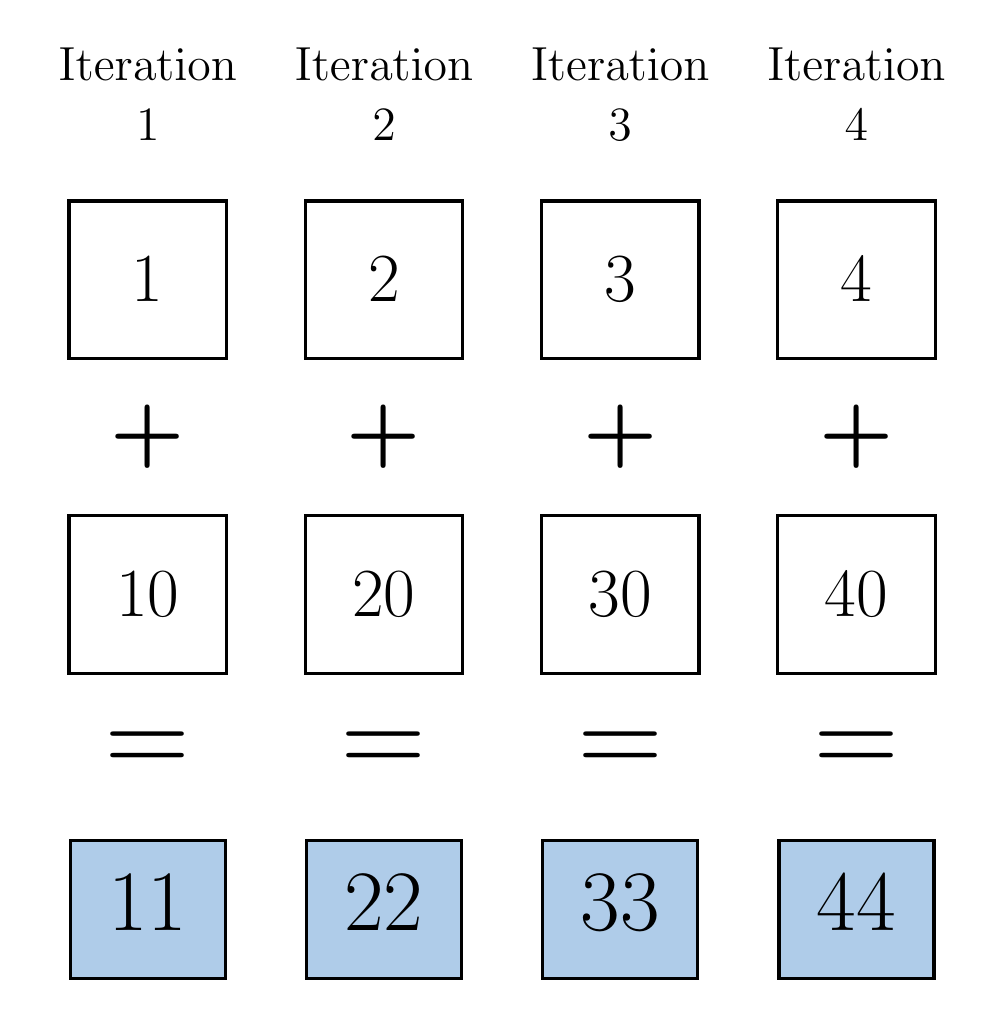
\begin{tikzpicture}

\tikzstyle{square} = [draw,outer sep=5,inner sep=3,minimum size=10,
    line width=0, very thick, draw=black!100,
    top color=white,bottom color=white]
\tikzstyle{blue} = [draw=black!100,outer sep=5,inner sep=5,line width=1,
very thick, minimum width=10, minimum height=10, 
top color=myblue, bottom color=myblue, scale=1.25, font=\Huge]

% =========================
% four scalars - first row
% =========================
\draw[square] (9,10.5) rectangle (11,12.5);
\node at (10,11.5) {\Huge 1};
\node[scale=1.2] at (10,13.8) {\Large \begin{tabular}{c} Iteration \\ 1\end{tabular}};

\draw[square] (12,10.5) rectangle (14,12.5);
\node at (13,11.5) {\Huge 2};
\node[scale=1.2] at (13,13.8) {\Large \begin{tabular}{c} Iteration \\ 2\end{tabular}};

\draw[square] (15,10.5) rectangle (17,12.5);
\node at (16,11.5) {\Huge 3};
\node[scale=1.2] at (16,13.8) {\Large \begin{tabular}{c} Iteration \\ 3\end{tabular}};

\draw[square] (18,10.5) rectangle (20,12.5);
\node at (19,11.5) {\Huge 4};
\node[scale=1.2]at (19,13.8) {\Large \begin{tabular}{c} Iteration \\ 4\end{tabular}};

% =========================
% four scalars - second row
% =========================
\draw[square] (9,6.5) rectangle (11,8.5);
\node at (10,7.5) {\Huge 10};


\draw[square] (12,6.5) rectangle (14,8.5);
\node at (13,7.5) {\Huge 20};


\draw[square] (15,6.5) rectangle (17,8.5);
\node at (16,7.5) {\Huge 30};


\draw[square] (18,6.5) rectangle (20,8.5);
\node at (19,7.5) {\Huge 40};


% plus signs between vector 1 and vector 2
\node[scale=3] at (10,9.5) {\textbf{+}};
\node[scale=3] at (13,9.5) {\textbf{+}};
\node[scale=3] at (16,9.5) {\textbf{+}};
\node[scale=3] at (19,9.5) {\textbf{+}};

% =========================
% Down arrows
% =========================
\node[scale=4] at (10,5.5) {\textbf{$=$}};
\node[scale=4] at (13,5.5) {\textbf{$=$}};
\node[scale=4] at (16,5.5) {\textbf{$=$}};
\node[scale=4] at (19,5.5) {\textbf{$=$}};

% =========================
% % four scalars - results
% =========================
\node[blue] at (10,3.5) {\begin{tabular}{c} 11 \end{tabular}};
\node[blue] at (13,3.5) {\begin{tabular}{c} 22 \end{tabular}};
\node[blue] at (16,3.5) {\begin{tabular}{c} 33 \end{tabular}};
\node[blue] at (19,3.5) {\begin{tabular}{c} 44 \end{tabular}};


\end{tikzpicture}
\end{document}

